\documentclass{article}
\usepackage[spanish]{babel}
\usepackage[utf8]{inputenc}
\usepackage{authblk}
\usepackage{url}
\usepackage{graphicx}

\title{Fundamentos Estadísticos - Trabajo Final}

\author{Martin A. Miguel (\texttt{mmiguel@dc.uba.ar})}
\affil{Lic. en Cs de la Computación - Laboratorio de Inteligencia Artificial
Aplicada, Depto. de Computación, Fac. de Cs. Exactas y Naturales, Univ. de
Buenos Aires, Buenos Aires, Argentina}

\date{31 de Julio de 2017}

\begin{document}

\maketitle

\section{Marco Teórico}

\subsection{Tema de investigación}

Mi tema de investigación de doctorado consiste en el modelado de la inferencia
de estructuras jerárquicas que realizan las personas sobre eventos en el
tiempo. La investigación se centra principalmente en la inferencia de
estructuras jerárquicas en la música, ya que es de nuestro particular interés y
es un caso claro y estudiable de cómo las personas realizan esta tarea. Cuando
hablamos de estructuras jerárquicas nos referimos a descripciones de la
secuencia de eventos mediante agrupaciones de los eventos en grupos relevantes,
que pueden a si mismo ser agrupados. Un ejemplo de esto es como en la
poesía las palabras se agrupan en versos y luego en estrofas. 

Nuestra investigación se apoya en la idea de que la comunicación entre
personas se basa mucho en estas estructuras y que mucha de la información
necesaria para inferir las mismas se encuentra en la distribución de
los eventos en el tiempo. El objetivo de investigación es construir modelos
computacionales que observando información temporal de los eventos puedan
generar estructuras jerárquicas cognitivamente relevantes.

Por otra parte soy partícipe de un grupo de investigación que busca aplicar
herramientas de machine learning a análisis de música y composición
automática. 

\subsection{Datos y música}

En el presente trabajo proponemos trabajar analizando las duraciones de 
notas en un dataset de improvisaciones de jazz. El dataset utilizado es el
\textbf{Weimar Jazz Dataset} \url{http://jazzomat.hfm-weimar.de/index.html}.
Este dataset contiene la información de 456 improvisaciones clasificadas en
distintos estilos dentro del Jazz. Como parte de la introducción presentaremos
conceptos de música que servirán para comprender los datos analizados.

\subsubsection{Música}

Una canción o interpretación musical puede definirse por cuándo suena qué
cosa. De esta manera, hay varias formas de describir una canción. La
descripción tradicional es la de una partitura musical escrita sobre un
pentagrama (ver fig \ref{fig:part}).

\begin{figure}[h]
\centering
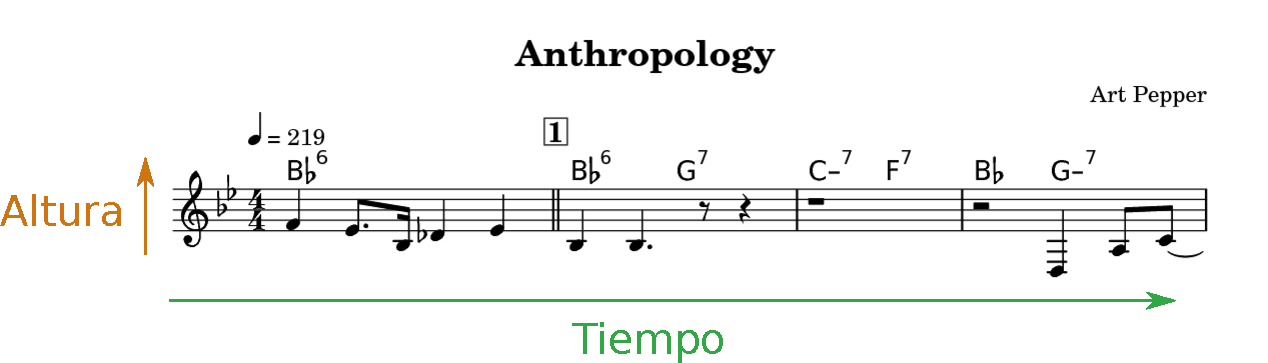
\includegraphics[width=\textwidth]{graficos/partitura.pdf}
\caption{Ejemplo de una partitura}\label{fig:part}
\end{figure}

En una partitura se busca explicitar la información de los eventos musicales.
Cada bolita representa un evento musical. La disposición en vertical describe
la altura de la nota (que tan grave o aguda suena) y la disposición horizontal
describe cuando suena respecto del principio de la canción.

Otra visualización de una canción es el \emph{piano roll} (ver fig
\ref{fig:piano_roll}). Nuevamente, el eje vertical es la altura de la nota y
el eje horizontal es el tiempo. Cada cuadrado representa un evento musical y
su largo representa su duración.

\begin{figure}[h]
\centering
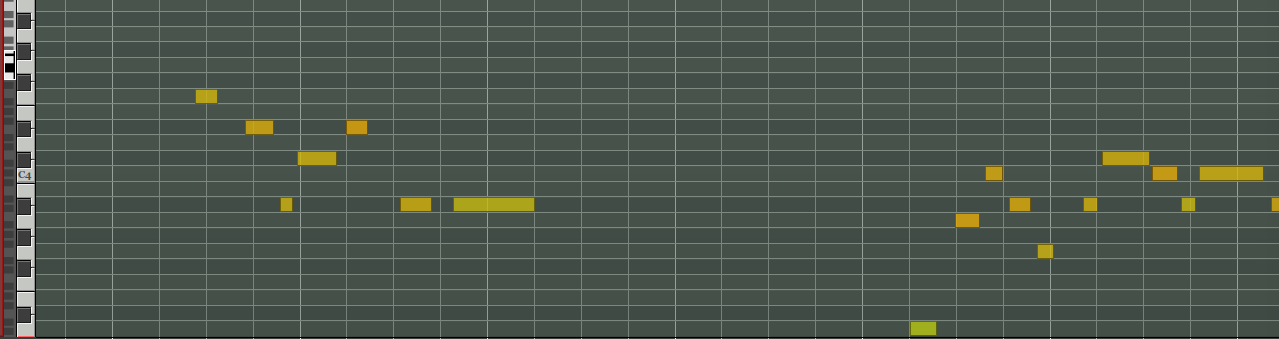
\includegraphics[width=\textwidth]{graficos/piano_roll.png}
\caption{Visualización en formato \emph{piano roll} de la
canción}\label{fig:piano_roll}
\end{figure}

\section{Lista de Ejercicios}

\section{Resolución}

\section{Justificación}

\end{document}
